\documentclass[../main.tex]{subfiles}
\begin{document}

\ifSubfilesClassLoaded{
	\mainmatter
	\setcounter{chapter}{5}
}{}

\chapter{Results}
\label{ch:result}
\section{Drell-Yan Cross Section Ratio}
\pdfmargincomment{run 5-6 compared with 2-3 and full data set}

\subsection{Intensity extrapolation}

\subsection{Mass fit result}

\subsection{Extraction of \texorpdfstring{$\bar{d}/\bar{u}$}{dbar/ubar}}
The $\sigma_{pd}/2\sigma_{pp}$ ratio is used by the NNPDF collaboration in
their PDF extraction\cite{ball2021} and their result is shown in Fig.\
\ref{fig:nnpdf_e906}.

\begin{figure}[htbp!]
	\centering
	\begin{subfigure}{0.45\linewidth}
		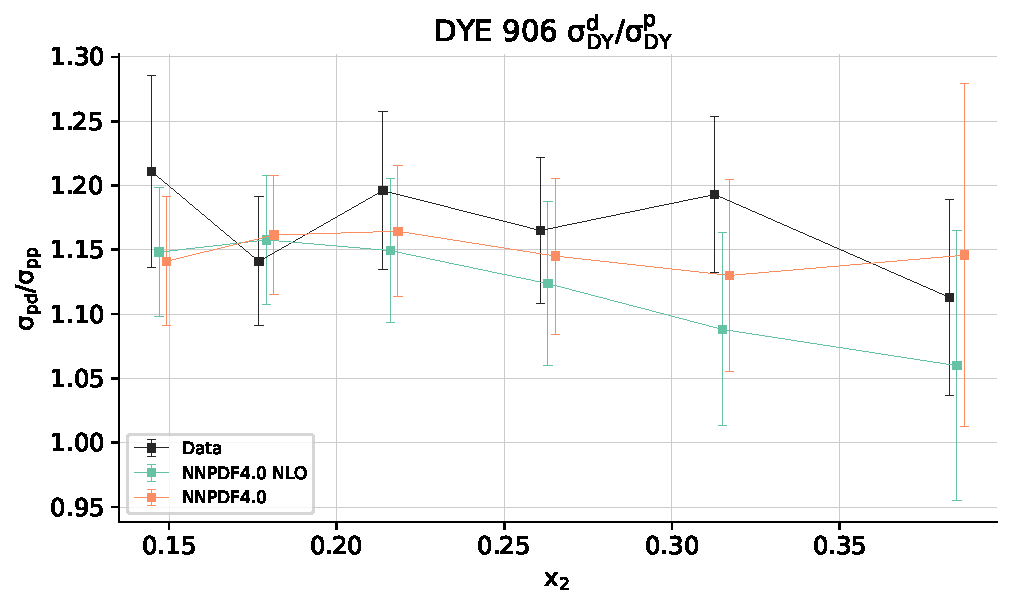
\includegraphics[width=\linewidth]{data_vs_theory_nnpdf40_e906}
		\caption{Calculated Drell-Yan cross section ratio.}
		\label{subfig:nnpdf_e906_csr}
	\end{subfigure}
	\begin{subfigure}{0.45\linewidth}
		
\includegraphics[width=\linewidth]{placeholder}
		\caption{Extracted $\bar{d/}\bar{u}$ ratio.}
		\label{subfig:nnpdf_e906_x2}
	\end{subfigure}
	\caption{Comparison of NNPDF4.0\cite{ball2021} with the SeaQuest
		result\cite{dove2021}.}
	\label{fig:nnpdf_e906}
	\pdfmargincomment{Should be compared with the new result from run5-6 and full
		data set}
\end{figure}

\pdfmargincomment{comment on the effect from the target contamination correction}

\section{Charmonium Cross Section}
\pdfmargincomment{absolute cross section and cross section ratios; mean pT for
	jpsi as a function of root s}


The massfits in each $x_F$ bins are shown in \cref{fig:massfit_57-70_xF,fig:massfit_5-6_xF},
and the fit in the $P_T$ bins are shown in \cref{fig:massfit_57-70_pT,fig:massfit_5-6_pT}.
The two datasets are analyzed separately. The data in each bin is very well described by the fitting procedure
and the $J/\psi$ and $\psi'$ yield can be extracted from the massfits.
\begin{figure}[h]
	\centering
	\begin{subfigure}{0.4\linewidth}
		\includegraphics[width=0.9\linewidth]{massfit/run2-3/LH2/xF/LH2_xFbin0}
	\end{subfigure}
	\begin{subfigure}{0.4\linewidth}
		\includegraphics[width=0.9\linewidth]{massfit/run2-3/LD2/xF/LD2_xFbin0}
	\end{subfigure}\\
	\begin{subfigure}{0.4\linewidth}
		\includegraphics[width=0.9\linewidth]{massfit/run2-3/LH2/xF/LH2_xFbin1}
	\end{subfigure}
	\begin{subfigure}{0.4\linewidth}
		\includegraphics[width=0.9\linewidth]{massfit/run2-3/LD2/xF/LD2_xFbin1}
	\end{subfigure}\\
	\begin{subfigure}{0.4\linewidth}
		\includegraphics[width=0.9\linewidth]{massfit/run2-3/LH2/xF/LH2_xFbin2}
	\end{subfigure}
	\begin{subfigure}{0.4\linewidth}
		\includegraphics[width=0.9\linewidth]{massfit/run2-3/LD2/xF/LD2_xFbin2}
	\end{subfigure}\\
	\begin{subfigure}{0.4\linewidth}
		\includegraphics[width=0.9\linewidth]{massfit/run2-3/LH2/xF/LH2_xFbin3}
	\end{subfigure}
	\begin{subfigure}{0.4\linewidth}
		\includegraphics[width=0.9\linewidth]{massfit/run2-3/LD2/xF/LD2_xFbin3}
	\end{subfigure}\\
	\begin{subfigure}{0.4\linewidth}
		\includegraphics[width=0.9\linewidth]{massfit/run2-3/LH2/xF/LH2_xFbin4}
	\end{subfigure}
	\begin{subfigure}{0.4\linewidth}
		\includegraphics[width=0.9\linewidth]{massfit/run2-3/LD2/xF/LD2_xFbin4}
	\end{subfigure}
	\caption{Mass fit for run 2-3 data in each $x_F$ bin for both \ce{LH_2}(left) and \ce{LD_2}(right) targets. }
	\label{fig:massfit_57-70_xF}
\end{figure}

\begin{figure}[h]
	\centering
	\begin{subfigure}{0.4\linewidth}
		\includegraphics[width=0.9\linewidth]{massfit/run5-6/LH2/xF/LH2_xFbin0}
	\end{subfigure}
	\begin{subfigure}{0.4\linewidth}
		\includegraphics[width=0.9\linewidth]{massfit/run5-6/LD2/xF/LD2_xFbin0}
	\end{subfigure}\\
	\begin{subfigure}{0.4\linewidth}
		\includegraphics[width=0.9\linewidth]{massfit/run5-6/LH2/xF/LH2_xFbin1}
	\end{subfigure}
	\begin{subfigure}{0.4\linewidth}
		\includegraphics[width=0.9\linewidth]{massfit/run5-6/LD2/xF/LD2_xFbin1}
	\end{subfigure}\\
	\begin{subfigure}{0.4\linewidth}
		\includegraphics[width=0.9\linewidth]{massfit/run5-6/LH2/xF/LH2_xFbin2}
	\end{subfigure}
	\begin{subfigure}{0.4\linewidth}
		\includegraphics[width=0.9\linewidth]{massfit/run5-6/LD2/xF/LD2_xFbin2}
	\end{subfigure}\\
	\begin{subfigure}{0.4\linewidth}
		\includegraphics[width=0.9\linewidth]{massfit/run5-6/LH2/xF/LH2_xFbin3}
	\end{subfigure}
	\begin{subfigure}{0.4\linewidth}
		\includegraphics[width=0.9\linewidth]{massfit/run5-6/LD2/xF/LD2_xFbin3}
	\end{subfigure}\\
	\begin{subfigure}{0.4\linewidth}
		\includegraphics[width=0.9\linewidth]{massfit/run5-6/LH2/xF/LH2_xFbin4}
	\end{subfigure}
	\begin{subfigure}{0.4\linewidth}
		\includegraphics[width=0.9\linewidth]{massfit/run5-6/LD2/xF/LD2_xFbin4}
	\end{subfigure}
	\caption{Mass fit for run 5-6 data in each $x_F$ bin for both \ce{LH_2}(left) and \ce{LD_2}(right) targets. }
	\label{fig:massfit_5-6_xF}
\end{figure}

\begin{figure}[h]
	\centering
	\begin{subfigure}{0.4\linewidth}
		\includegraphics[width=0.9\linewidth]{massfit/run2-3/LH2/pT/LH2_pTbin0}
	\end{subfigure}
	\begin{subfigure}{0.4\linewidth}
		\includegraphics[width=0.9\linewidth]{massfit/run2-3/LD2/pT/LD2_pTbin0}
	\end{subfigure}\\
	\begin{subfigure}{0.4\linewidth}
		\includegraphics[width=0.9\linewidth]{massfit/run2-3/LH2/pT/LH2_pTbin1}
	\end{subfigure}
	\begin{subfigure}{0.4\linewidth}
		\includegraphics[width=0.9\linewidth]{massfit/run2-3/LD2/pT/LD2_pTbin1}
	\end{subfigure}\\
	\begin{subfigure}{0.4\linewidth}
		\includegraphics[width=0.9\linewidth]{massfit/run2-3/LH2/pT/LH2_pTbin2}
	\end{subfigure}
	\begin{subfigure}{0.4\linewidth}
		\includegraphics[width=0.9\linewidth]{massfit/run2-3/LD2/pT/LD2_pTbin2}
	\end{subfigure}\\
	\begin{subfigure}{0.4\linewidth}
		\includegraphics[width=0.9\linewidth]{massfit/run2-3/LH2/pT/LH2_pTbin3}
	\end{subfigure}
	\begin{subfigure}{0.4\linewidth}
		\includegraphics[width=0.9\linewidth]{massfit/run2-3/LD2/pT/LD2_pTbin3}
	\end{subfigure}\\
	\begin{subfigure}{0.4\linewidth}
		\includegraphics[width=0.9\linewidth]{massfit/run2-3/LH2/pT/LH2_pTbin4}
	\end{subfigure}
	\begin{subfigure}{0.4\linewidth}
		\includegraphics[width=0.9\linewidth]{massfit/run2-3/LD2/pT/LD2_pTbin4}
	\end{subfigure}
	\caption{Mass fit for run 2-3 data in each $P_T$ bin for both \ce{LH_2}(left) and \ce{LD_2}(right) targets. }
	\label{fig:massfit_57-70_pT}
\end{figure}

\begin{figure}[h]
	\centering
	\begin{subfigure}{0.4\linewidth}
		\includegraphics[width=0.9\linewidth]{massfit/run5-6/LH2/pT/LH2_pTbin0}
	\end{subfigure}
	\begin{subfigure}{0.4\linewidth}
		\includegraphics[width=0.9\linewidth]{massfit/run5-6/LD2/pT/LD2_pTbin0}
	\end{subfigure}\\
	\begin{subfigure}{0.4\linewidth}
		\includegraphics[width=0.9\linewidth]{massfit/run5-6/LH2/pT/LH2_pTbin1}
	\end{subfigure}
	\begin{subfigure}{0.4\linewidth}
		\includegraphics[width=0.9\linewidth]{massfit/run5-6/LD2/pT/LD2_pTbin1}
	\end{subfigure}\\
	\begin{subfigure}{0.4\linewidth}
		\includegraphics[width=0.9\linewidth]{massfit/run5-6/LH2/pT/LH2_pTbin2}
	\end{subfigure}
	\begin{subfigure}{0.4\linewidth}
		\includegraphics[width=0.9\linewidth]{massfit/run5-6/LD2/pT/LD2_pTbin2}
	\end{subfigure}\\
	\begin{subfigure}{0.4\linewidth}
		\includegraphics[width=0.9\linewidth]{massfit/run5-6/LH2/pT/LH2_pTbin3}
	\end{subfigure}
	\begin{subfigure}{0.4\linewidth}
		\includegraphics[width=0.9\linewidth]{massfit/run5-6/LD2/pT/LD2_pTbin3}
	\end{subfigure}\\
	\begin{subfigure}{0.4\linewidth}
		\includegraphics[width=0.9\linewidth]{massfit/run5-6/LH2/pT/LH2_pTbin4}
	\end{subfigure}
	\begin{subfigure}{0.4\linewidth}
		\includegraphics[width=0.9\linewidth]{massfit/run5-6/LD2/pT/LD2_pTbin4}
	\end{subfigure}
	\caption{Mass fit for run 5-6 data in each $P_T$ bin for both \ce{LH_2}(left) and \ce{LD_2}(right) targets. }
	\label{fig:massfit_5-6_pT}
\end{figure}

With the yields extracted, the cross section can be calculated.
The branching ratios, $B\left(J/\psi\rightarrow\mu^+\mu-\right)$
and $B\left(\psi'\rightarrow\mu^+\mu-\right)$, are taken from Ref.~\cite{workman2022}.

\begin{figure}[h!]
	\centering
	\begin{subfigure}{0.45\linewidth}
		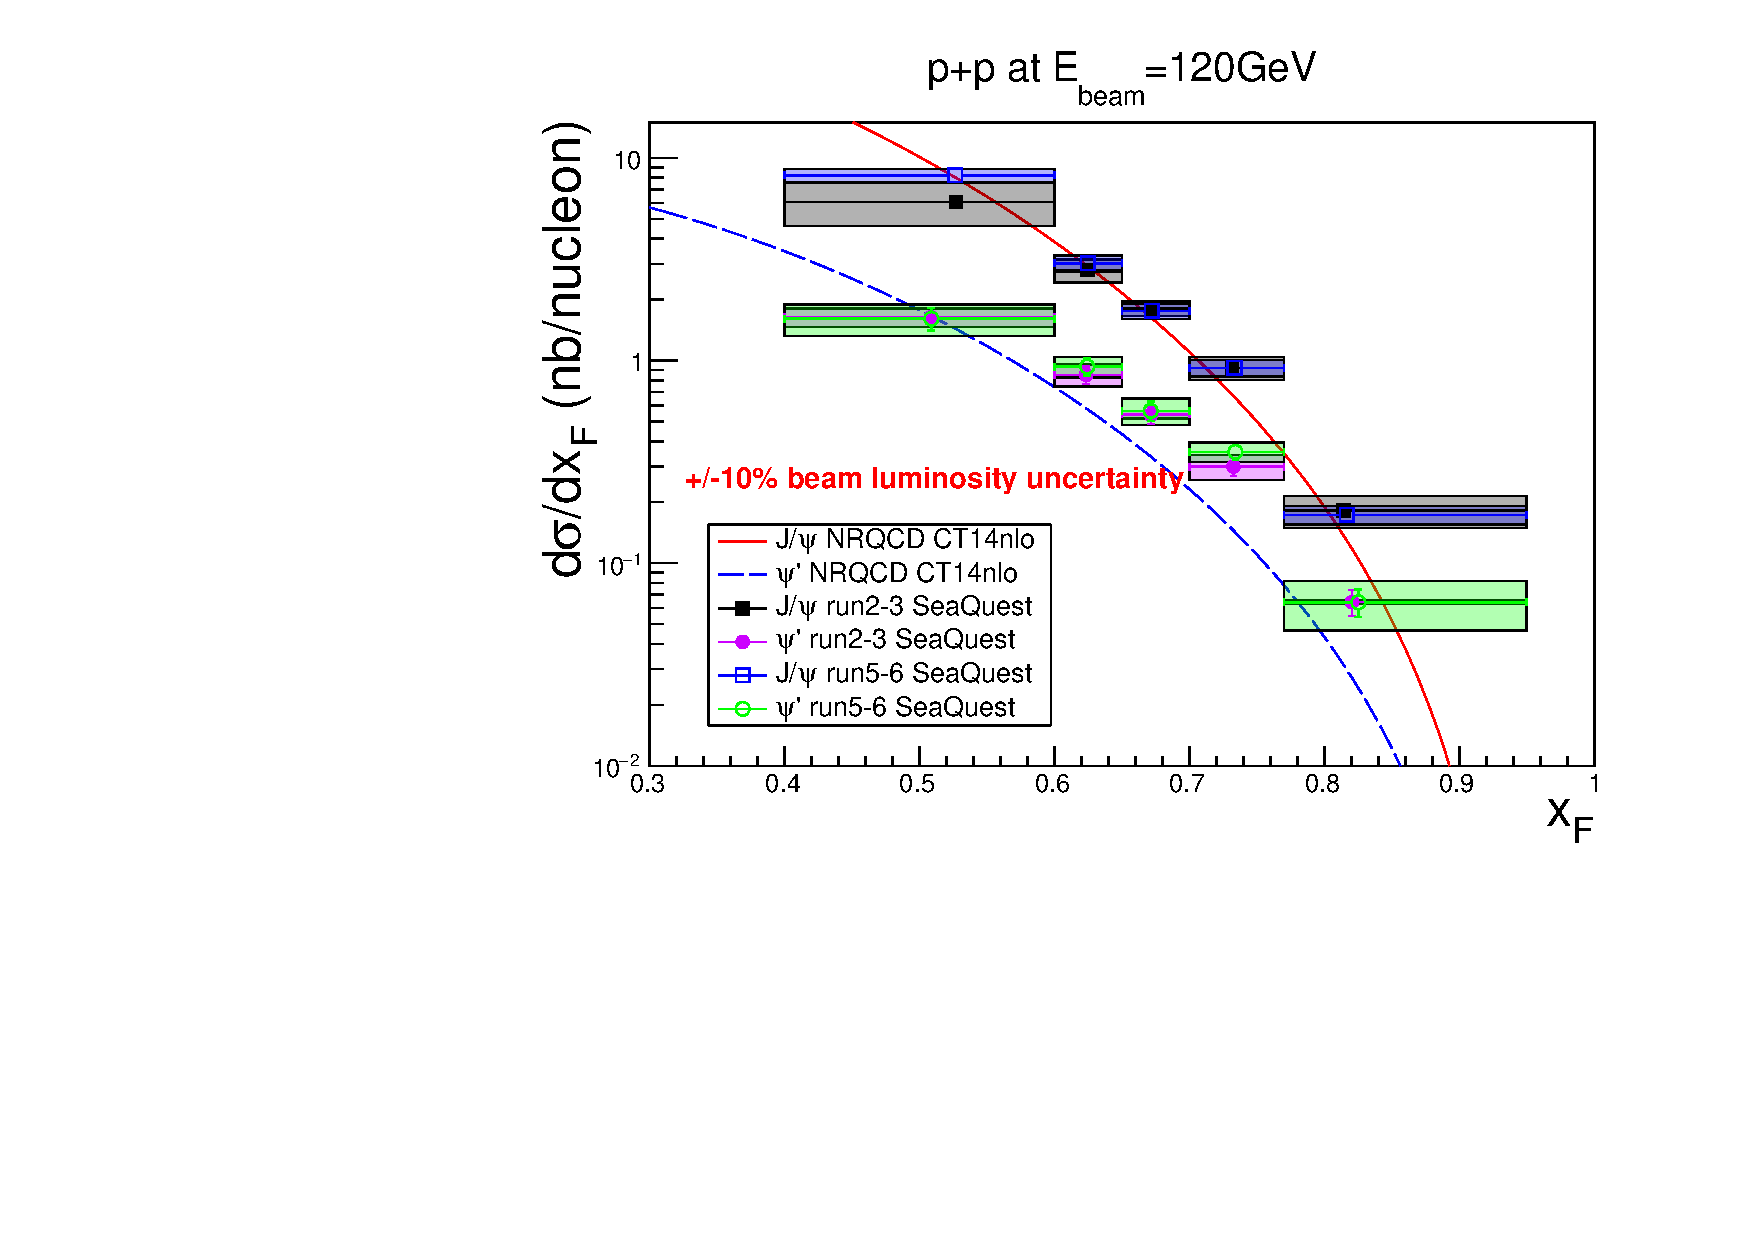
\includegraphics[width=0.9\linewidth]{cs/xF/combine_xF_LH2_5-6_5770_psip}
	\end{subfigure}
	\centering
	\begin{subfigure}{0.45\linewidth}
		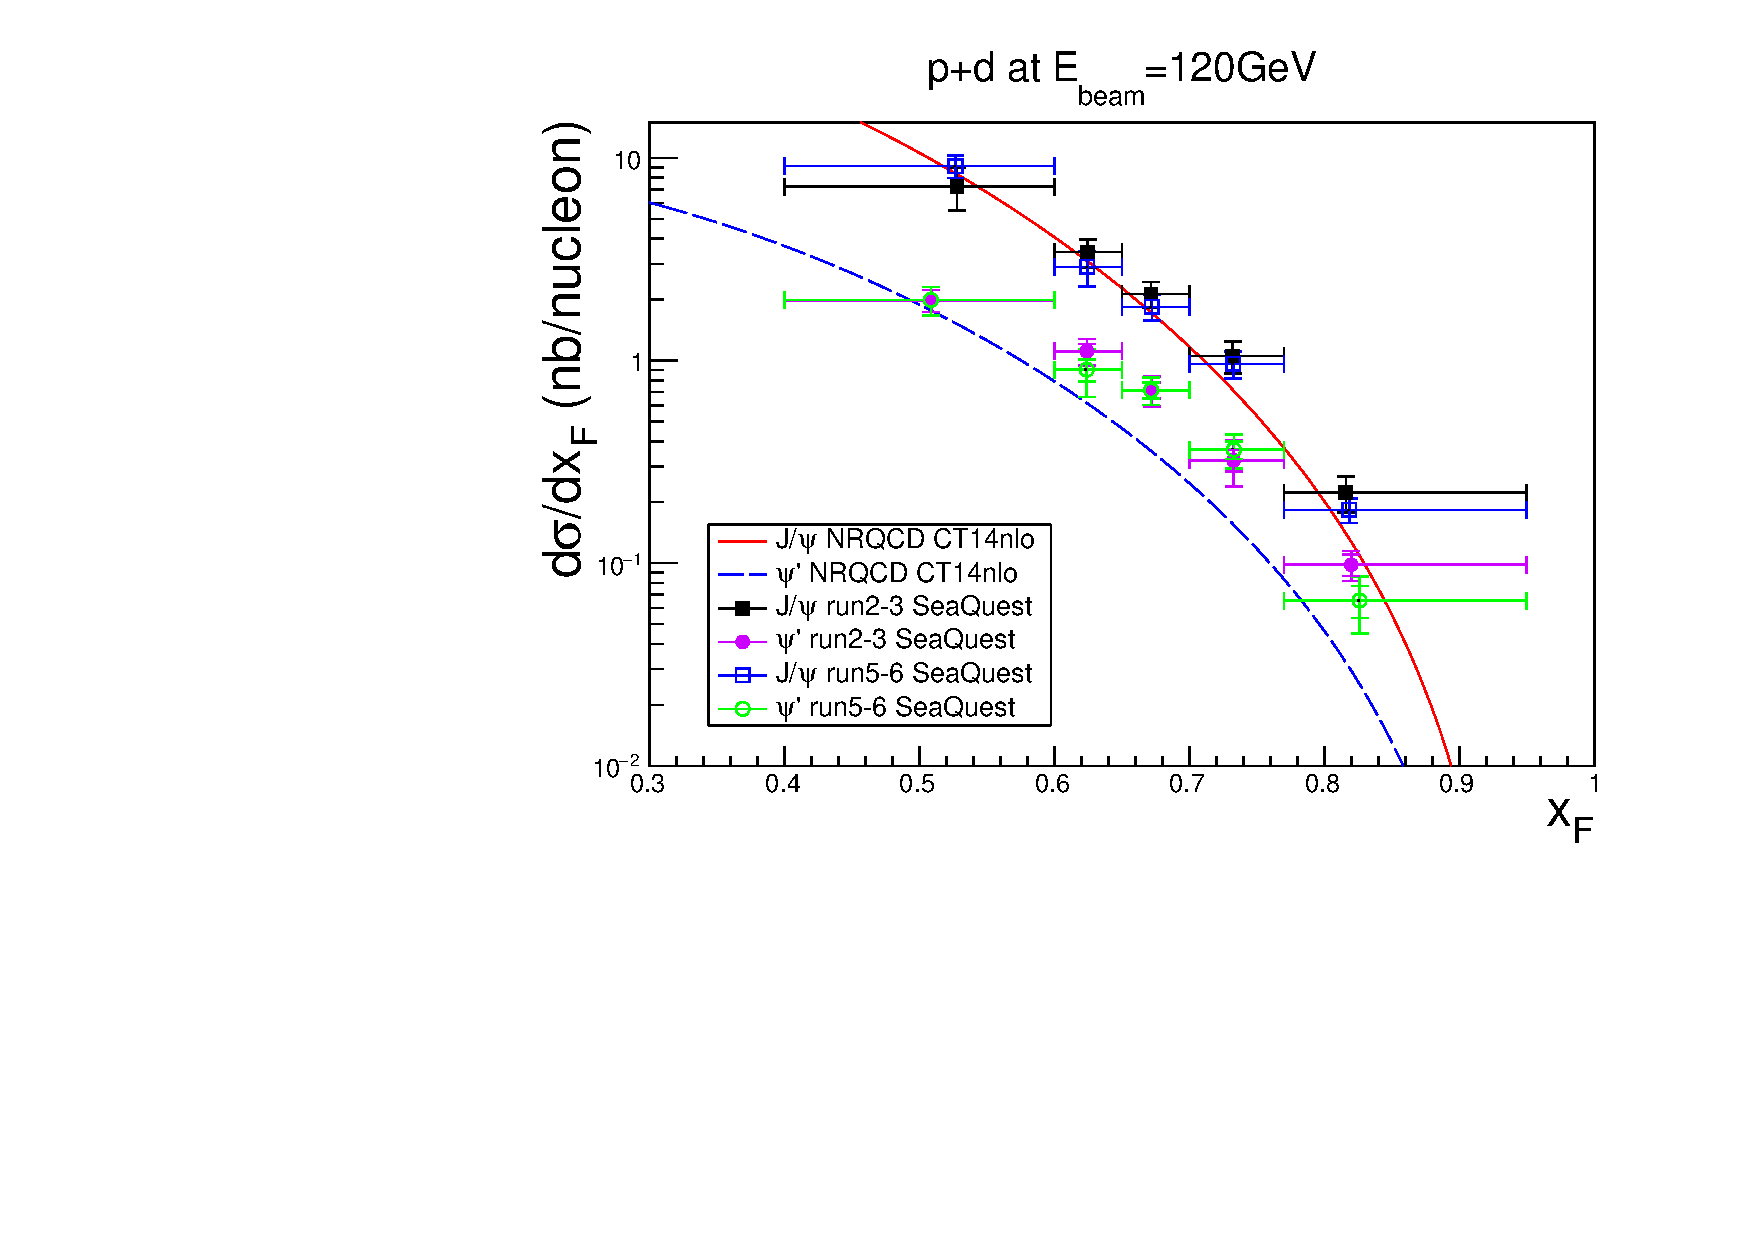
\includegraphics[width=0.9\linewidth]{cs/xF/combine_xF_LD2_5-6_5770_psip}
	\end{subfigure}
	\caption{The extracted $J/\psi$ and $\psi'$ cross section as a function of $x_F$ for $p+p$(left)
		and $p+d$(right) from the two datasets,	and compared with the NRQCD predictions}
	\label{fig:cs_xF_combined}
\end{figure}
\begin{figure}[h!]
	\centering
	\begin{subfigure}{0.45\linewidth}
		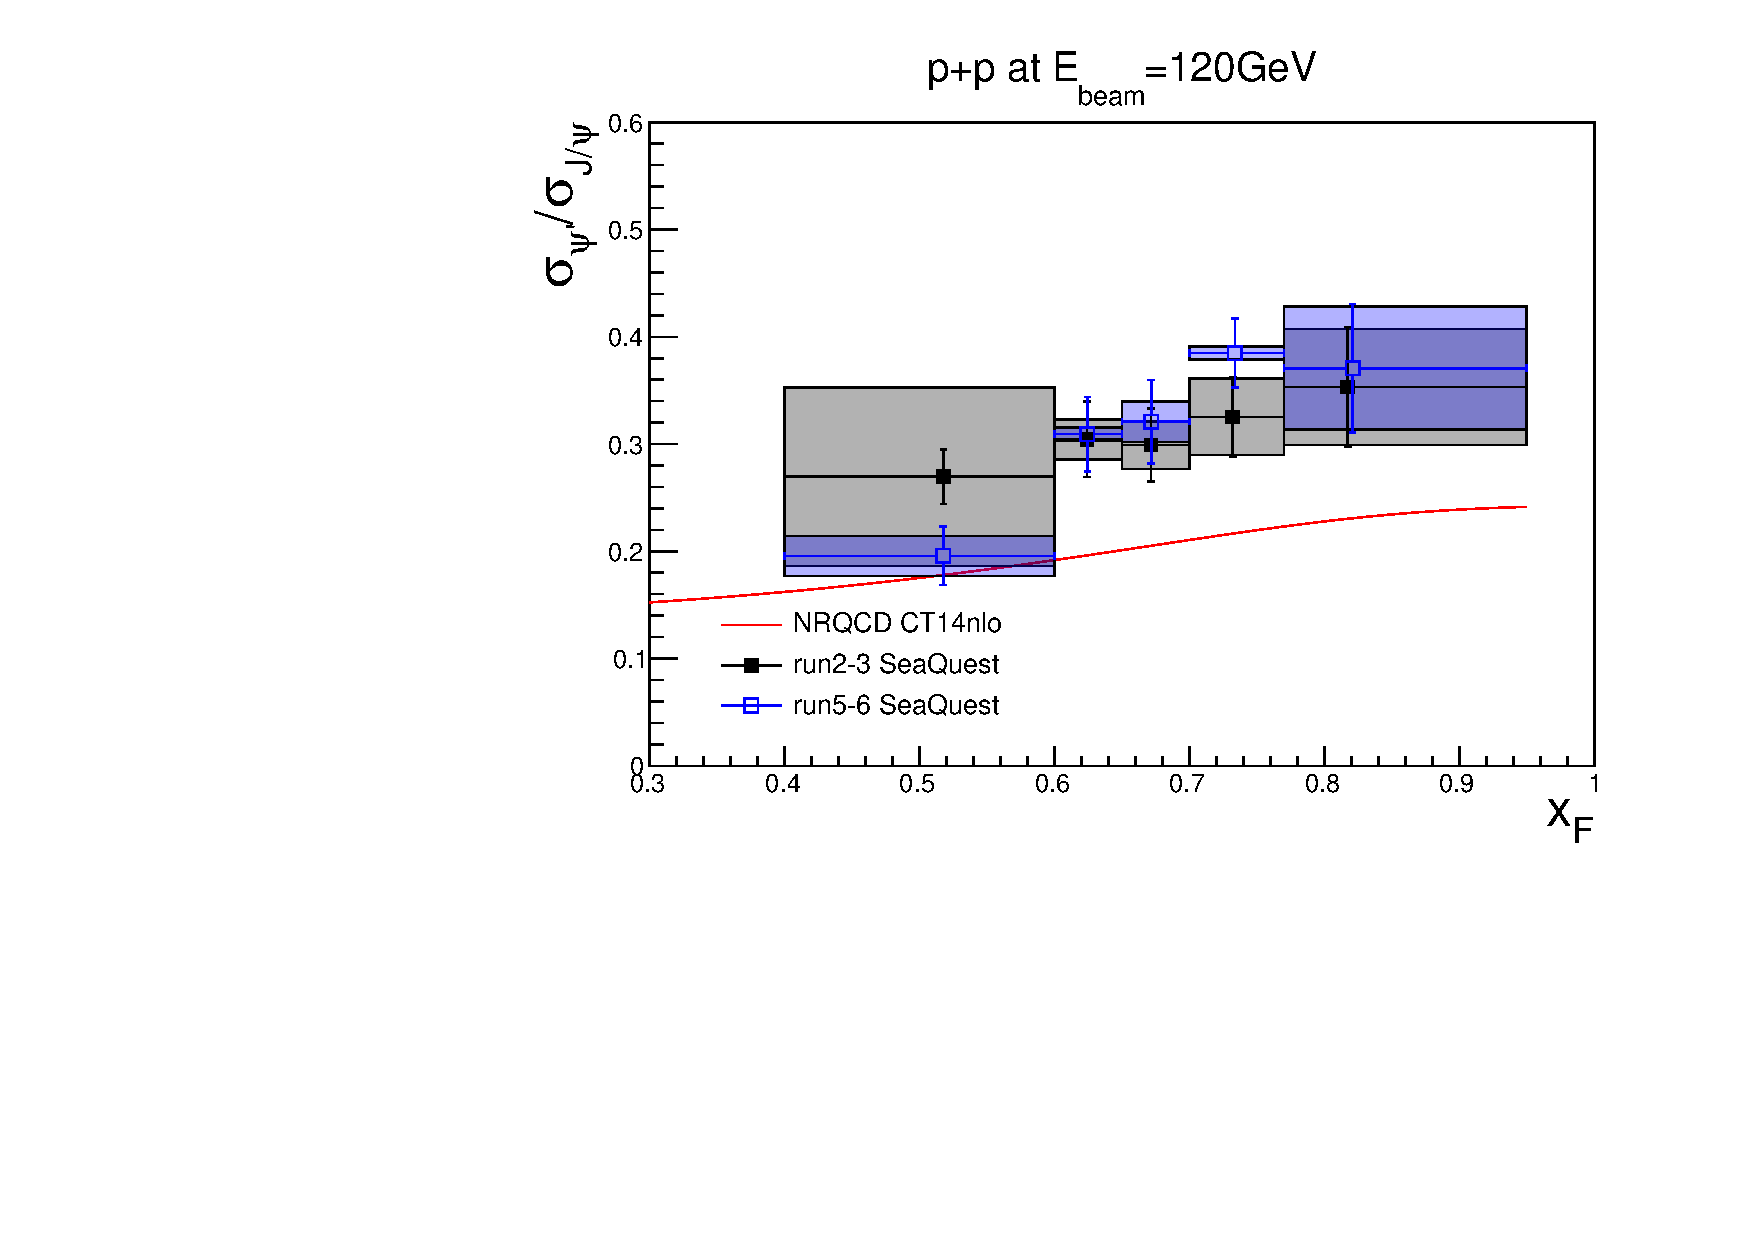
\includegraphics[width=0.9\linewidth]{cs/xF/ratio_xF_LH2_5-6_5770}
	\end{subfigure}
	\begin{subfigure}{0.45\linewidth}
		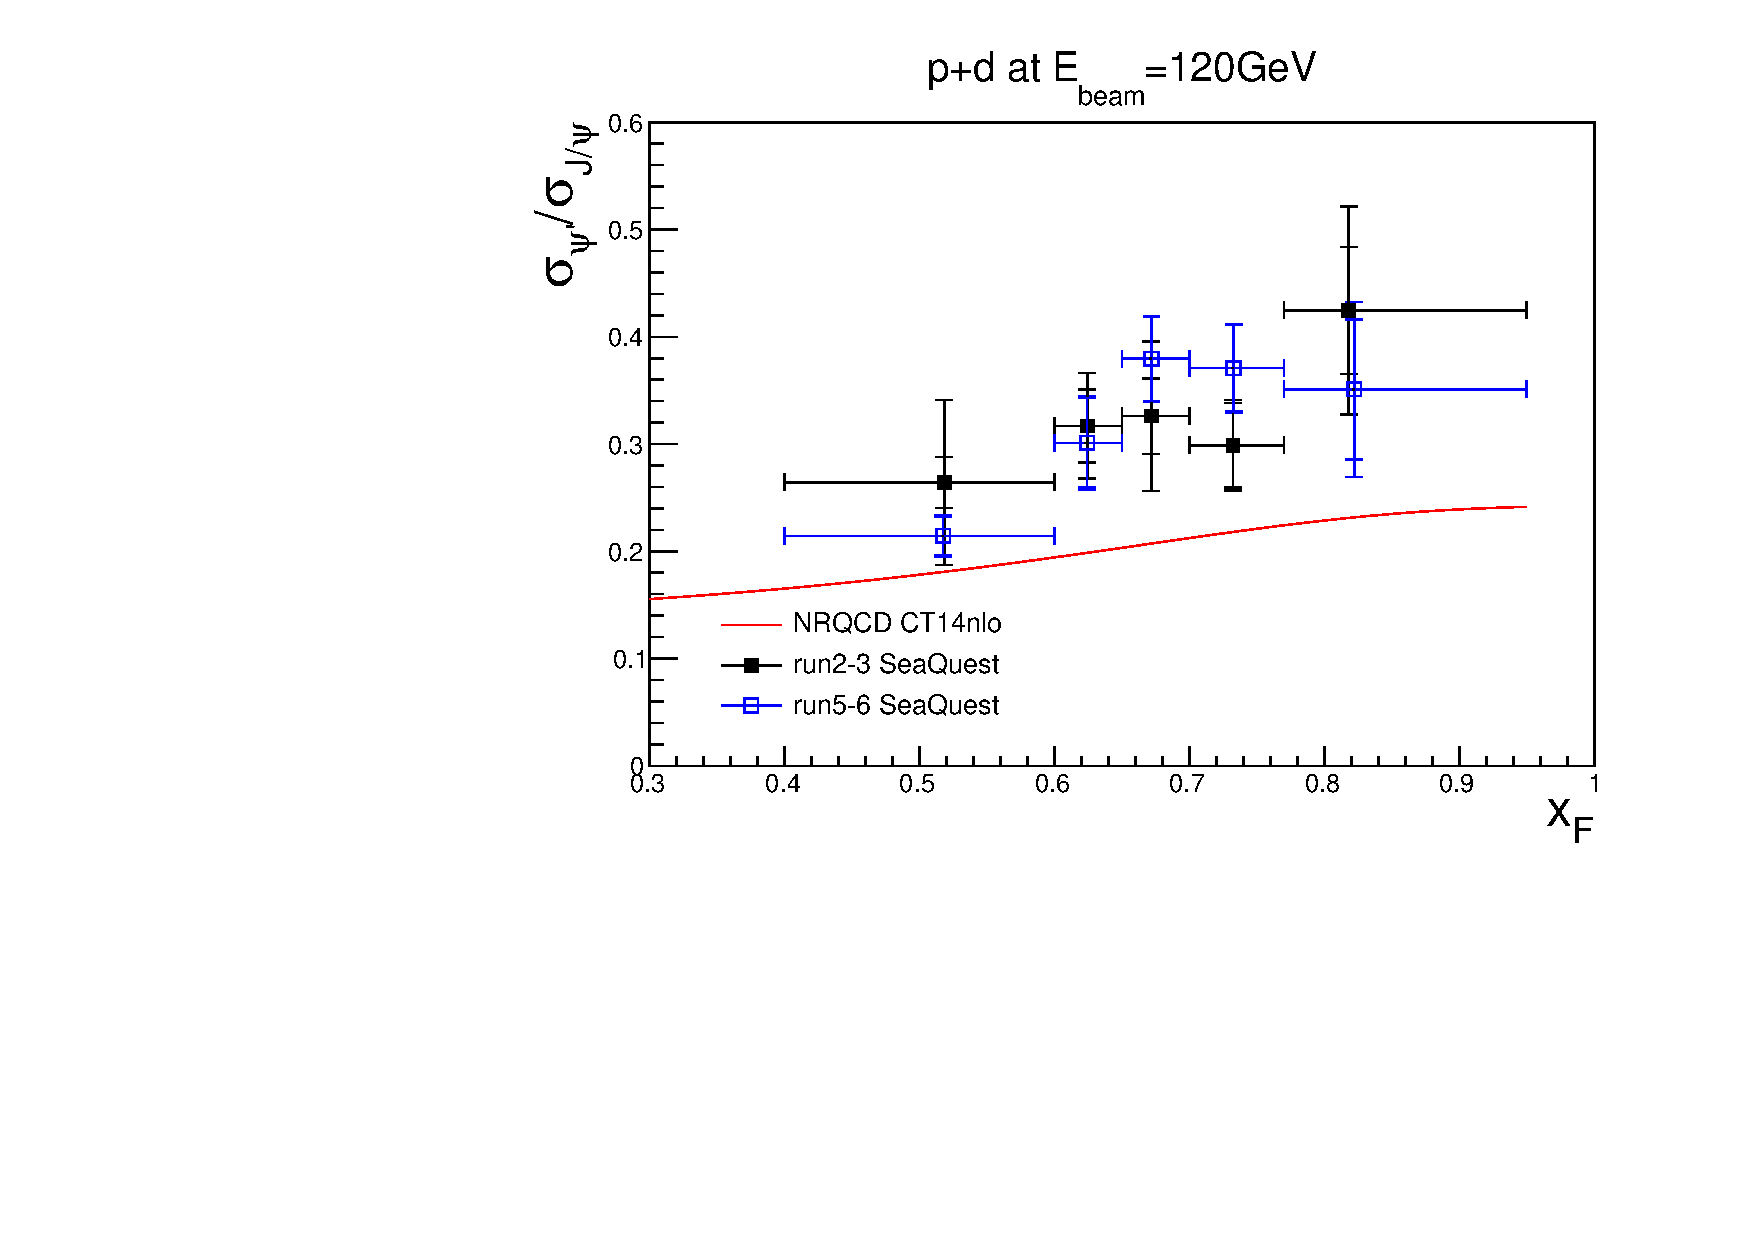
\includegraphics[width=0.9\linewidth]{cs/xF/ratio_xF_LD2_5-6_5770}
	\end{subfigure}
	\caption{The extracted  $\sigma_{\psi'}/\sigma_{J/\psi}$ ratio as a function of $x_F$ for $p+p$(left)
		and $p+d$(right) from the two datasets,	and compared with the NRQCD predictions}
\end{figure}

The extracted cross section for $J/\psi$ and $\psi'$ are shown in \cref{fig:cs_xF_combined}, and
the result from the two datasets are in very good agreement. While the extracted
$J/\psi$ cross section is in very good agreement with the NRQCD calculation, the extracted $\psi'$
cross section disagree with the prediction, particular at large $x_F$. It is possible the LDMEs used
in for the $\psi'$ cross section calculation is not fully optimized. This new result on the $\psi'$
cross section can be used in further constrain the LDMEs. In the NRQCD framework, the difference in the
$x_F$ distributions between $J/\psi$ and $\psi'$ is mostly originated from the relative weighting between
the different production subprocess. In the CEM framework, the hadronization probability only depends on
the final charmonium state, but not the underlying subprocess. Therefore, the CEM framework would predict
the $x_F$ distributions for $J/\psi$ and $\psi'$ to have very shape, with a smaller total cross section
for $\psi'$ production.


\begin{table}[h!]
	\centering
	\caption{Cross section as a function of $x_F$ (in \unit{\nano\barn\per nucleon}) for $p+p$ extracted from run 2-3, with their statistical and systematic uncertainties and the average $x_F$ in each bin.}
	\begin{tabular}{cc|ccc}
		\hline
		\multicolumn{2}{c|}{$J/\psi$} & \multicolumn{2}{c}{$\psi^{\prime}$} &                                                                      \\ \cline{1-4}
		$\expval{x_F}_{J/\psi}$       & $\eval{d\sigma/dx_F}_{J/\psi}$      & $\expval{x_F}_{\psi^\prime}$ & $\eval{d\sigma/dx_F}_{\psi^\prime}$ & \\ \cline{1-4}
		\multicolumn{1}{c|}{0.527}    & $6.070\pm0.333\pm1.465$             & \multicolumn{1}{c|}{0.509}   & $1.6362\pm0.1249\pm0.1692$          & \\
		\multicolumn{1}{c|}{0.625}    & $2.794\pm0.166\pm0.364$             & \multicolumn{1}{c|}{0.624}   & $0.8503\pm0.0841\pm0.1064$          & \\
		\multicolumn{1}{c|}{0.672}    & $1.810\pm0.100\pm0.154$             & \multicolumn{1}{c|}{0.672}   & $0.5414\pm0.0540\pm0.0230$          & \\
		\multicolumn{1}{c|}{0.732}    & $0.921\pm0.044\pm0.118$             & \multicolumn{1}{c|}{0.733}   & $0.2998\pm0.0307\pm0.0419$          & \\
		\multicolumn{1}{c|}{0.814}    & $0.182\pm0.011\pm0.032$             & \multicolumn{1}{c|}{0.821}   & $0.0642\pm0.0093\pm0.0012$          & \\ \cline{1-4}
	\end{tabular}
\end{table}
\begin{table}[h!]
	\centering
	\caption{Cross section as a function of $x_F$ (in \unit{\nano\barn\per nucleon}) for $p+d$ extracted from run 2-3, with their statistical and systematic uncertainties and the average $x_F$ in each bin.}
	\begin{tabular}{cc|ccc}
		\hline
		\multicolumn{2}{c|}{$J/\psi$} & \multicolumn{2}{c}{$\psi^{\prime}$} &                                                                      \\ \cline{1-4}
		$\expval{x_F}_{J/\psi}$       & $\eval{d\sigma/dx_F}_{J/\psi}$      & $\expval{x_F}_{\psi^\prime}$ & $\eval{d\sigma/dx_F}_{\psi^\prime}$ & \\ \cline{1-4}
		\multicolumn{1}{c|}{0.528}    & $6.626\pm0.361\pm1.457$             & \multicolumn{1}{c|}{0.509}   & $1.7513\pm0.1257\pm0.0613$          & \\
		\multicolumn{1}{c|}{0.625}    & $3.097\pm0.186\pm0.366$             & \multicolumn{1}{c|}{0.624}   & $0.9815\pm0.0869\pm0.0680$          & \\
		\multicolumn{1}{c|}{0.672}    & $1.912\pm0.114\pm0.183$             & \multicolumn{1}{c|}{0.672}   & $0.6232\pm0.0558\pm0.0596$          & \\
		\multicolumn{1}{c|}{0.732}    & $0.935\pm0.047\pm0.134$             & \multicolumn{1}{c|}{0.733}   & $0.2794\pm0.0341\pm0.0582$          & \\
		\multicolumn{1}{c|}{0.816}    & $0.189\pm0.013\pm0.030$             & \multicolumn{1}{c|}{0.820}   & $0.0802\pm0.0097\pm0.0043$          & \\ \cline{1-4}
	\end{tabular}
\end{table}
\begin{table}[h!]
	\centering
	\caption{Cross section as a function of $x_F$ (in \unit{\nano\barn\per nucleon}) for $p+p$ extracted from run 5-6, with their statistical and systematic uncertainties and the average $x_F$ in each bin.}
	\begin{tabular}{cc|ccc}
		\hline
		\multicolumn{2}{c|}{$J/\psi$} & \multicolumn{2}{c}{$\psi^{\prime}$} &                                                                      \\ \cline{1-4}
		$\expval{x_F}_{J/\psi}$       & $\eval{d\sigma/dx_F}_{J/\psi}$      & $\expval{x_F}_{\psi^\prime}$ & $\eval{d\sigma/dx_F}_{\psi^\prime}$ & \\ \cline{1-4}
		\multicolumn{1}{c|}{0.527}    & $8.219\pm0.458\pm0.616$             & \multicolumn{1}{c|}{0.509}   & $1.6087\pm0.2052\pm0.2854$          & \\
		\multicolumn{1}{c|}{0.625}    & $3.021\pm0.161\pm0.283$             & \multicolumn{1}{c|}{0.624}   & $0.9339\pm0.0918\pm0.1082$          & \\
		\multicolumn{1}{c|}{0.672}    & $1.759\pm0.087\pm0.151$             & \multicolumn{1}{c|}{0.671}   & $0.5647\pm0.0624\pm0.0845$          & \\
		\multicolumn{1}{c|}{0.733}    & $0.921\pm0.008\pm0.087$             & \multicolumn{1}{c|}{0.734}   & $0.3546\pm0.0293\pm0.0394$          & \\
		\multicolumn{1}{c|}{0.817}    & $0.173\pm0.008\pm0.018$             & \multicolumn{1}{c|}{0.825}   & $0.0641\pm0.0099\pm0.0177$          & \\ \cline{1-4}
	\end{tabular}
\end{table}
\begin{table}[h!]
	\centering
	\caption{Cross section as a function of $x_F$ (in \unit{\nano\barn\per nucleon}) for $p+d$ extracted from run 5-6, with their statistical and systematic uncertainties and the average $x_F$ in each bin.}
	\begin{tabular}{cc|ccc}
		\hline
		\multicolumn{2}{c|}{$J/\psi$} & \multicolumn{2}{c}{$\psi^{\prime}$} &                                                                      \\ \cline{1-4}
		$\expval{x_F}_{J/\psi}$       & $\eval{d\sigma/dx_F}_{J/\psi}$      & $\expval{x_F}_{\psi^\prime}$ & $\eval{d\sigma/dx_F}_{\psi^\prime}$ & \\ \cline{1-4}
		\multicolumn{1}{c|}{0.527}    & $9.184\pm0.378\pm0.579$             & \multicolumn{1}{c|}{0.509}   & $1.9688\pm0.1446\pm0.2002$          & \\
		\multicolumn{1}{c|}{0.624}    & $2.893\pm0.178\pm0.468$             & \multicolumn{1}{c|}{0.624}   & $0.8713\pm0.1083\pm0.1862$          & \\
		\multicolumn{1}{c|}{0.672}    & $1.834\pm0.089\pm0.171$             & \multicolumn{1}{c|}{0.672}   & $0.6963\pm0.0639\pm0.0523$          & \\
		\multicolumn{1}{c|}{0.733}    & $0.949\pm0.041\pm0.102$             & \multicolumn{1}{c|}{0.733}   & $0.3520\pm0.0355\pm0.0448$          & \\
		\multicolumn{1}{c|}{0.819}    & $0.180\pm0.008\pm0.015$             & \multicolumn{1}{c|}{0.826}   & $0.0630\pm0.0114\pm0.0147$          & \\ \cline{1-4}
	\end{tabular}
\end{table}


\pdfmargincomment{how to plot the pT distribution? Do I want to show jpsi and psi' on the same plot, or per roadset?}

The $P_T$ distribution is shown in \cref{fig:pT_57-70,fig:pT_5-6}
\begin{figure}[h!]
	\centering
	\begin{subfigure}{0.45\linewidth}
		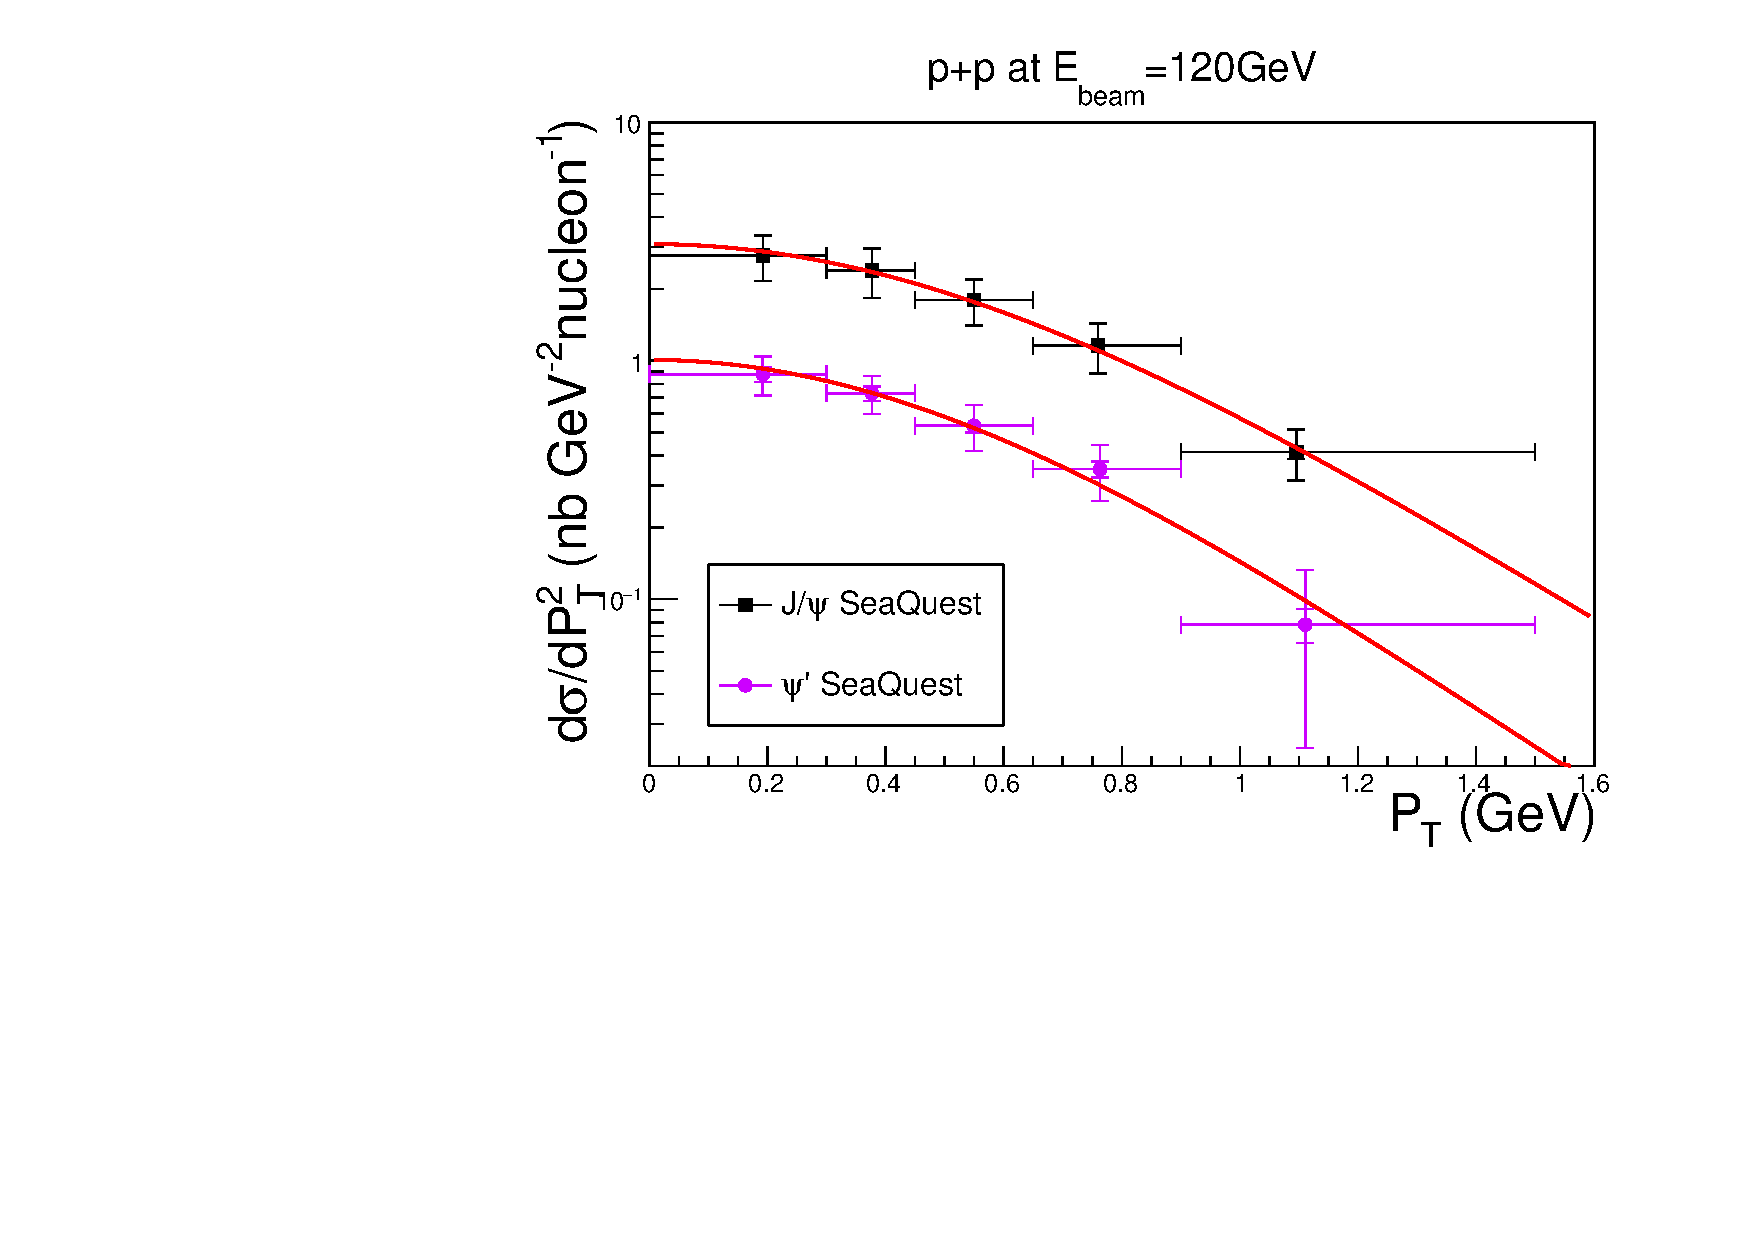
\includegraphics[width=0.9\linewidth]{cs/pT/57-70_pTsq_LH2}
	\end{subfigure}
	\begin{subfigure}{0.45\linewidth}
		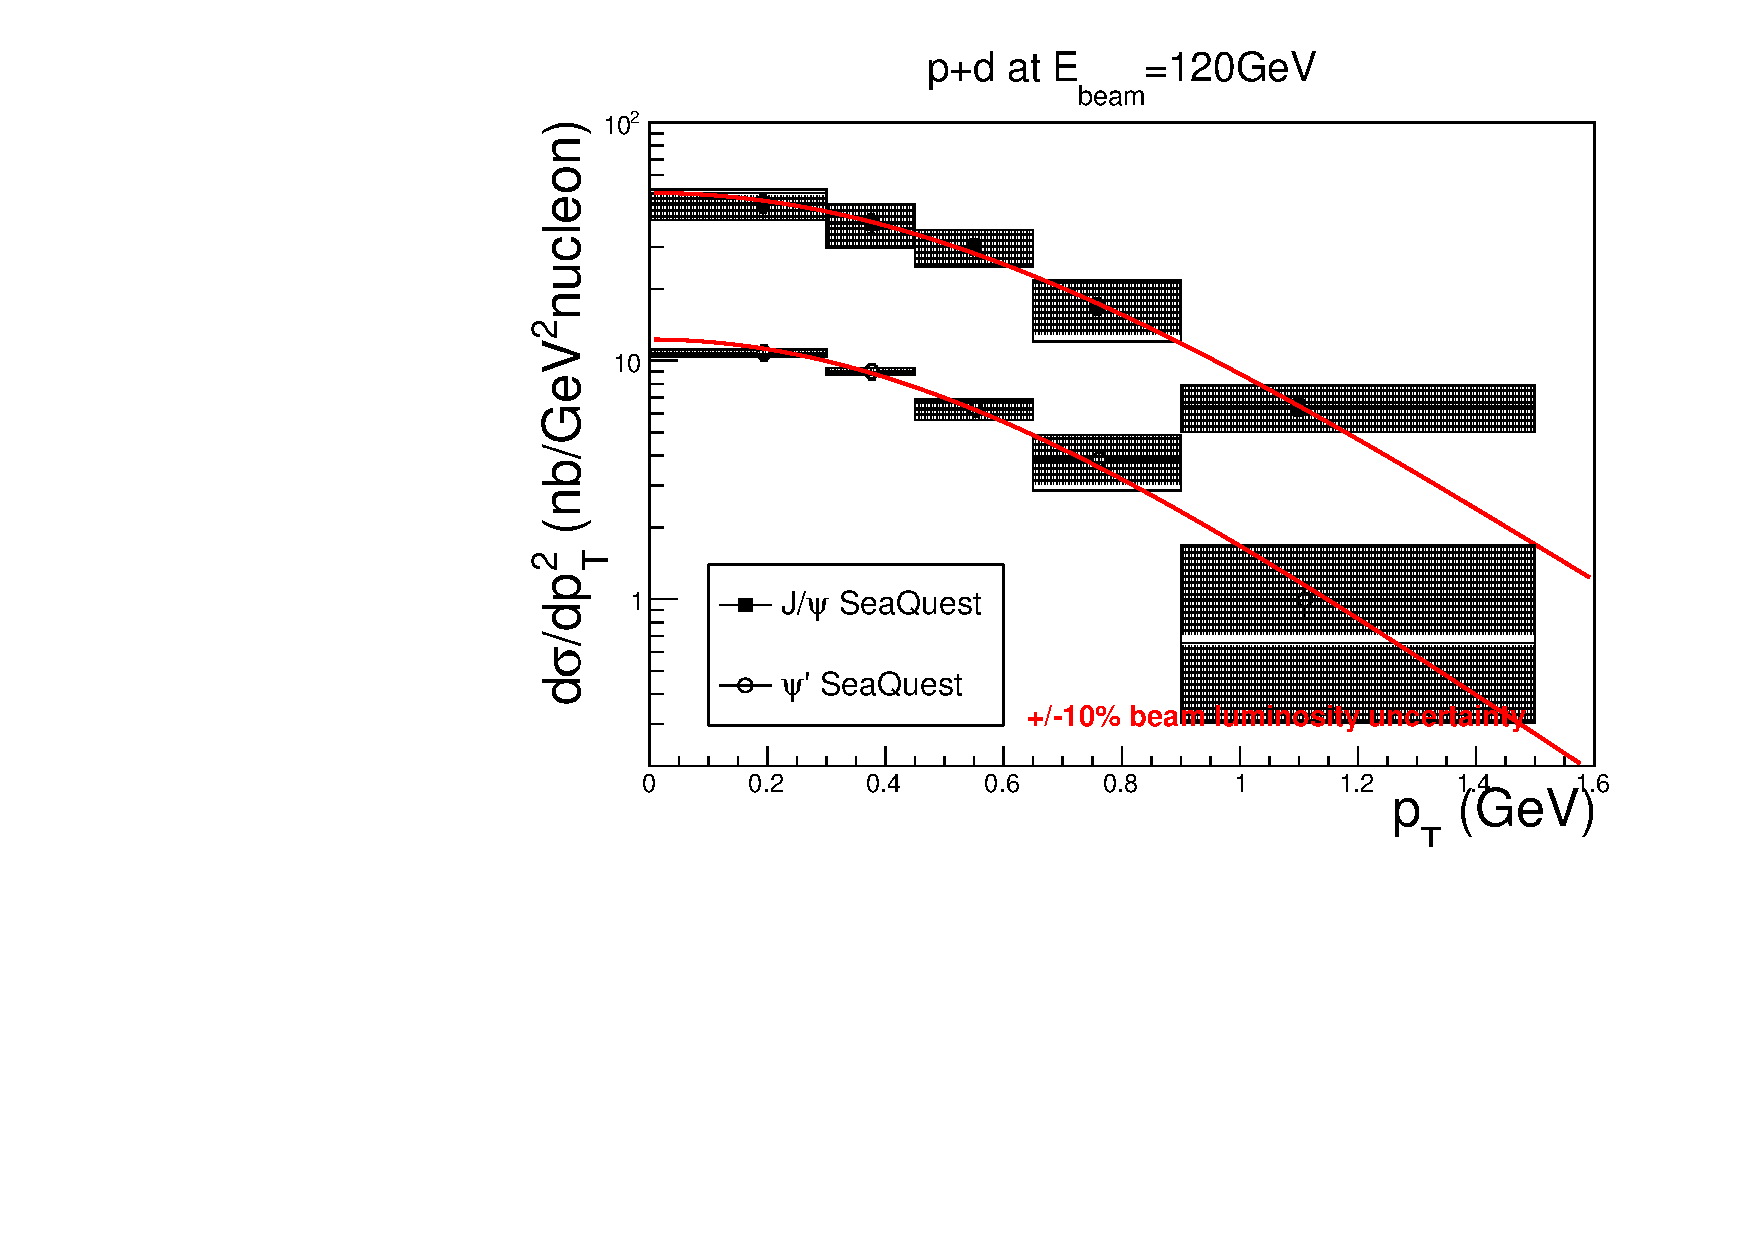
\includegraphics[width=0.9\linewidth]{cs/pT/57-70_pTsq_LD2}
	\end{subfigure}
	\caption{The extracted $J/\psi$ and $\psi'$ $P_T$ distribution for $p+p$(left)
		and $p+d$(right) from the run 2-3 data.}
	\label{fig:pT_57-70}
\end{figure}
\begin{figure}[h!]
	\centering
	\begin{subfigure}{0.45\linewidth}
		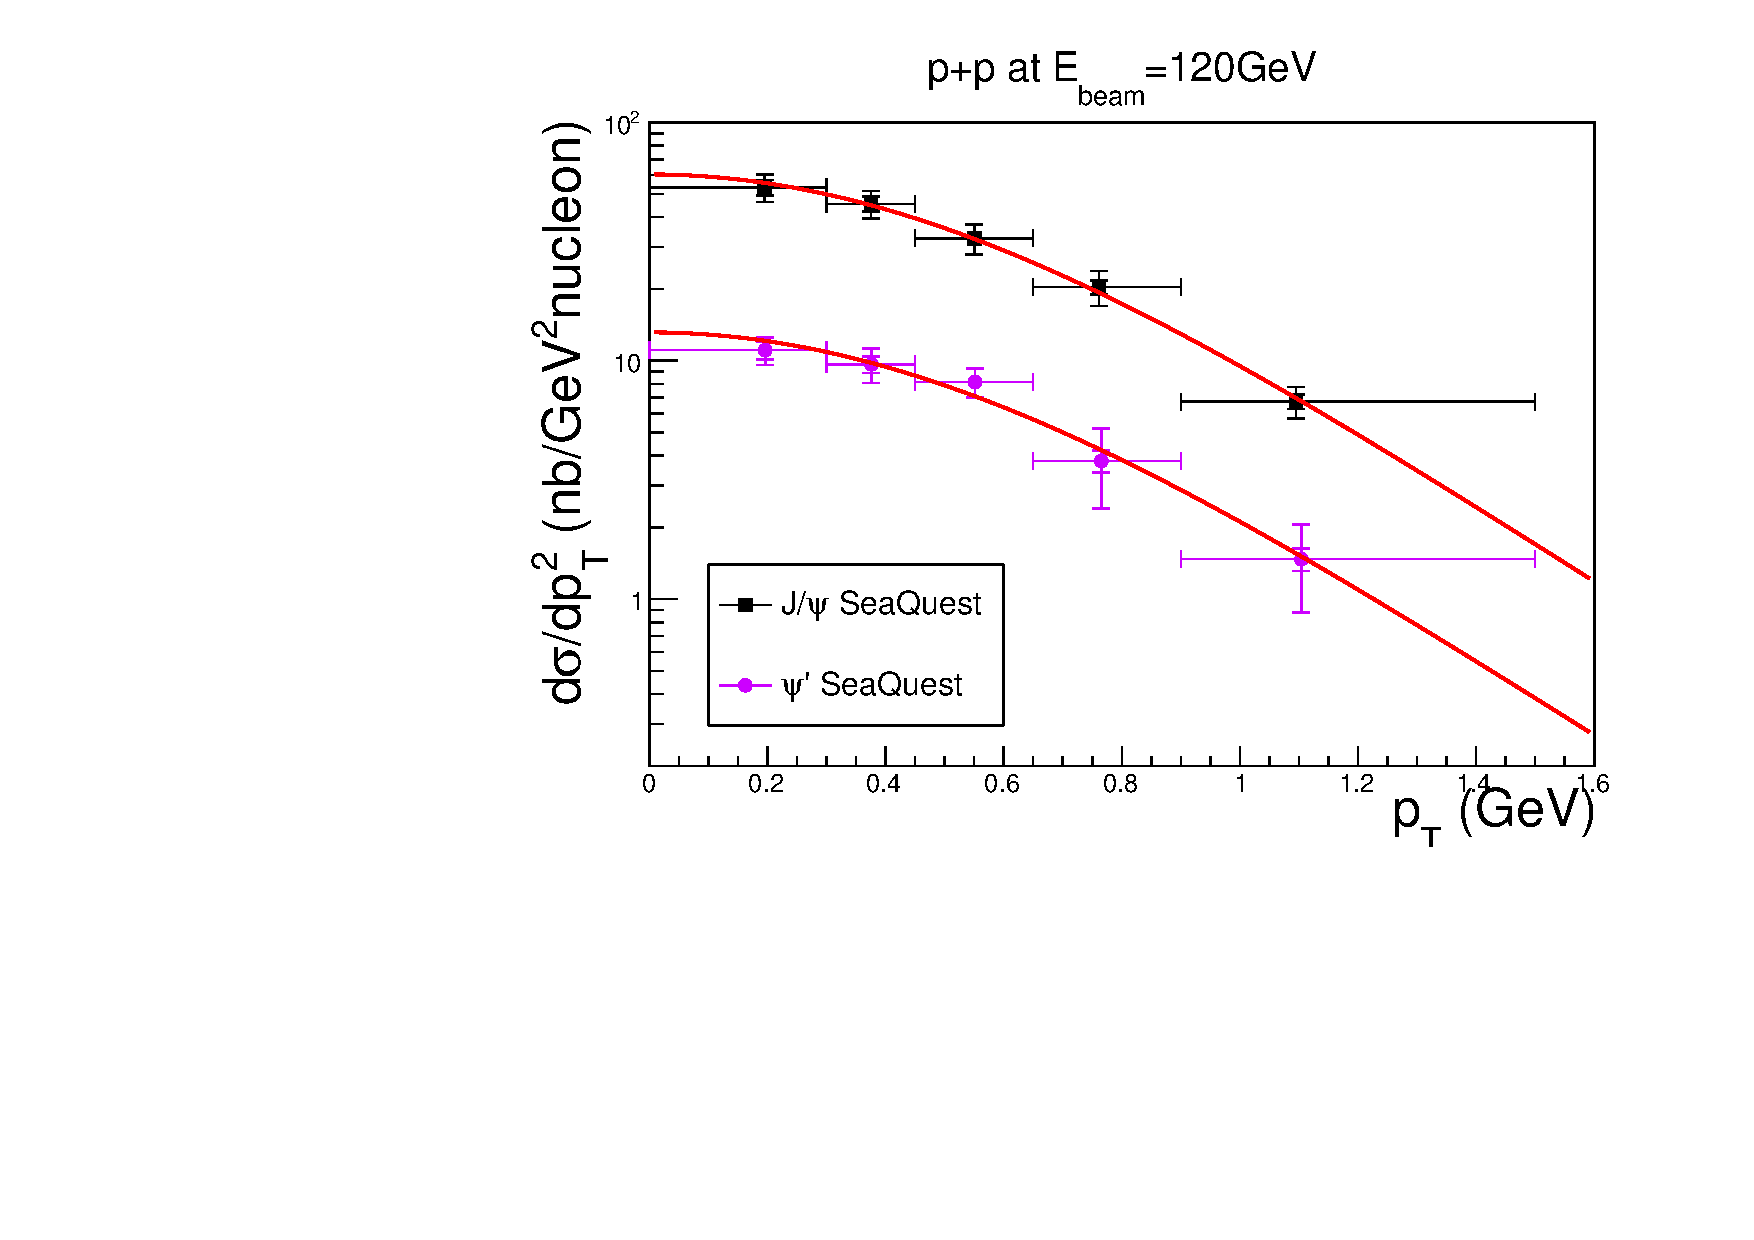
\includegraphics[width=0.9\linewidth]{cs/pT/5-6_pTsq_LH2}
	\end{subfigure}
	\begin{subfigure}{0.45\linewidth}
		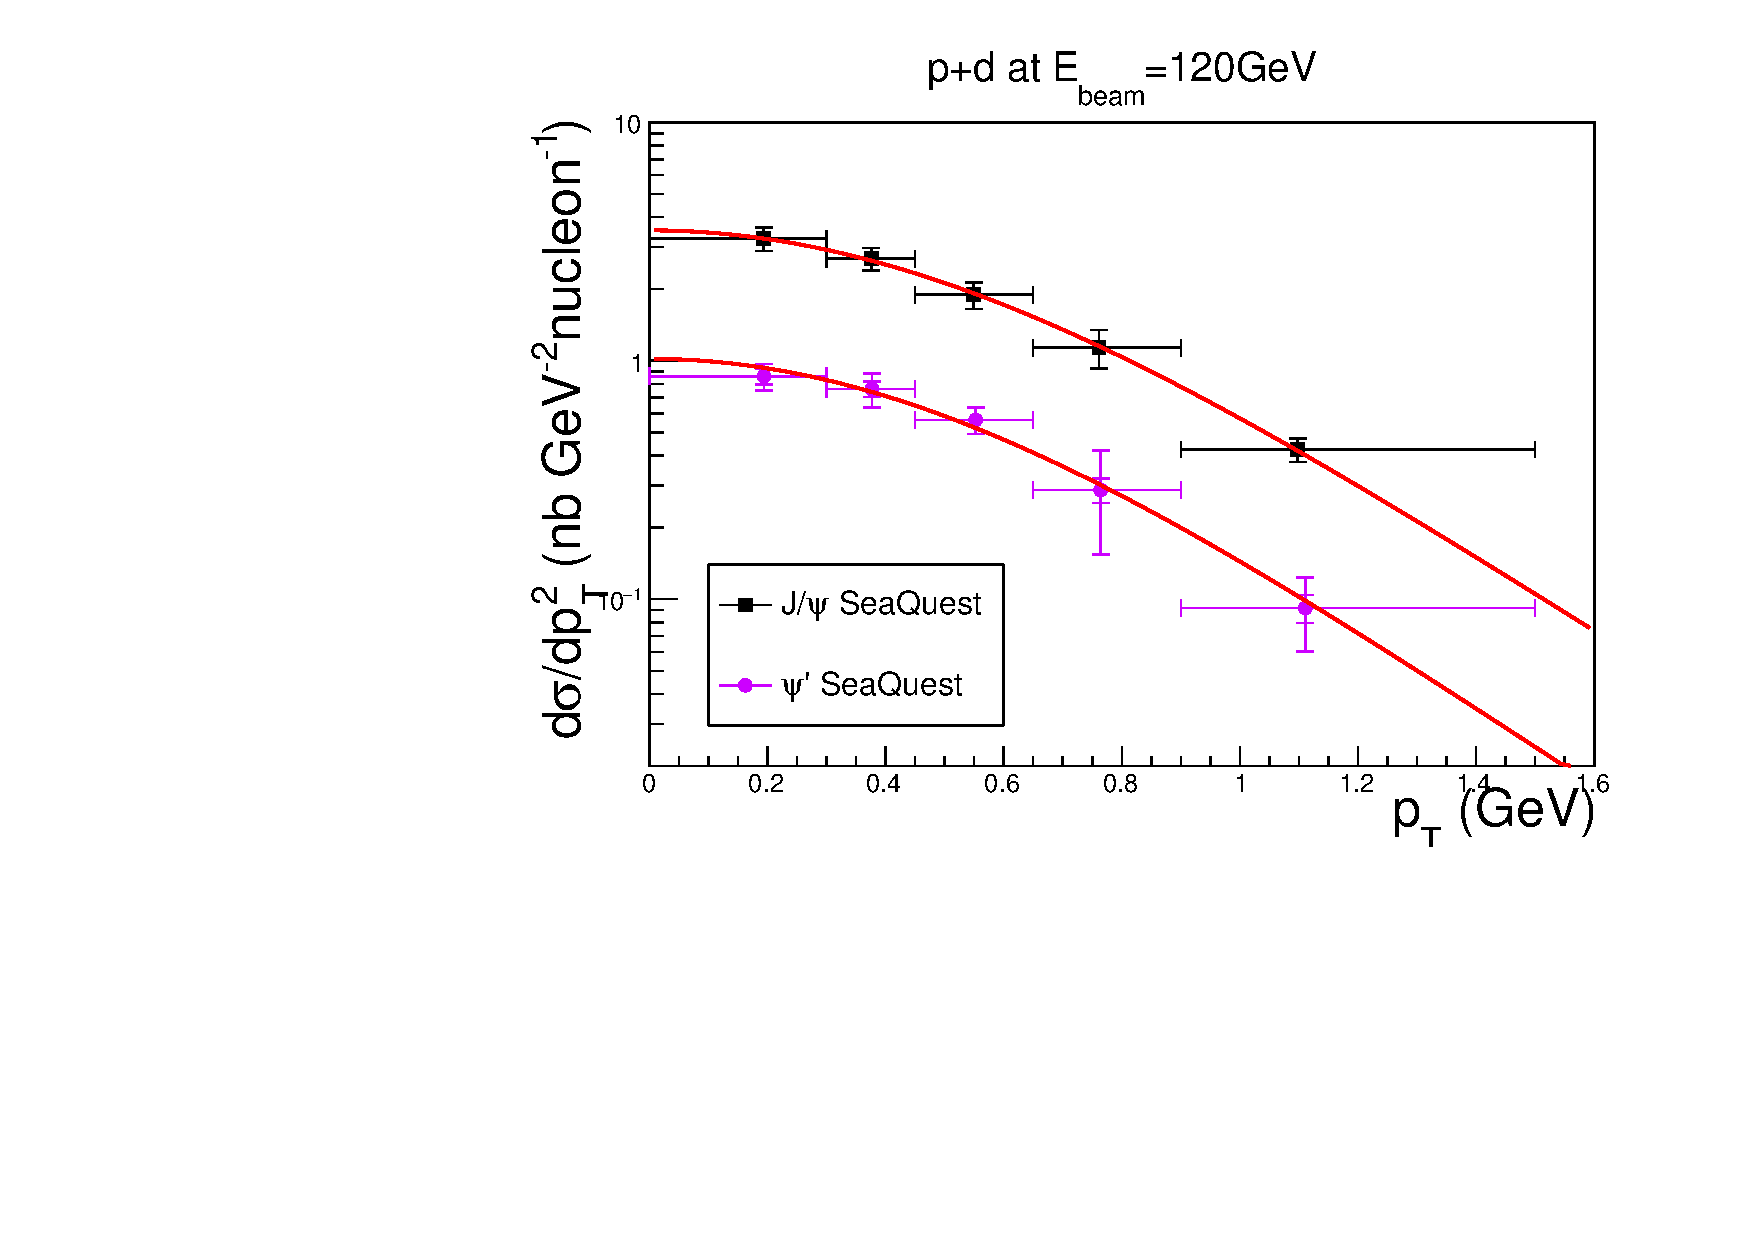
\includegraphics[width=0.9\linewidth]{cs/pT/5-6_pTsq_LD2}
	\end{subfigure}
	\caption{The extracted $J/\psi$ and $\psi'$ $P_T$ distribution for $p+p$(left)
		and $p+d$(right) from the run 2-3 data.}
	\label{fig:pT_5-6}
\end{figure}
\begin{figure}[h!]
	\centering
	\begin{subfigure}{0.45\linewidth}
		\includegraphics[width=0.9\linewidth]{cs/pT/ratio_pT_LH2_5-6_5770}
	\end{subfigure}
	\begin{subfigure}{0.45\linewidth}
		\includegraphics[width=0.9\linewidth]{cs/pT/ratio_pT_LD2_5-6_5770}
	\end{subfigure}
	\caption{The extracted  $\sigma_{\psi'}/\sigma_{J/\psi}$ ratio as a function of $P_T$ for $p+p$(left)
		and $p+d$(right) from the two datasets.}
\end{figure}
\begin{table}[h!]
	\centering
	\caption{The $\expval{p_T}$ (in \unit{\GeV}) and  $d\sigma/dp_T$ (in \unit{\nano\barn\GeV^{-1} nucleon^{-1}}) for $p+p$ extracted from run 2-3}
	\begin{tabular}{cc|ccc}
		\hline
		\multicolumn{2}{c|}{$J/\psi$} & \multicolumn{2}{c}{$\psi^{\prime}$} &                                                                      \\ \cline{1-4}
		$\expval{p_T}_{J/\psi}$       & $\eval{d\sigma/dp_T}_{J/\psi}$      & $\expval{p_T}_{\psi^\prime}$ & $\eval{d\sigma/dp_T}_{\psi^\prime}$ & \\ \cline{1-4}
		\multicolumn{1}{c|}{0.193}    & $12.65\pm1.07\pm2.40$               & \multicolumn{1}{c|}{0.192}   & $3.17\pm0.24\pm0.27$                & \\
		\multicolumn{1}{c|}{0.377}    & $27.68\pm2.43\pm5.48$               & \multicolumn{1}{c|}{0.377}   & $6.65\pm0.49\pm0.66$                & \\
		\multicolumn{1}{c|}{0.549}    & $30.22\pm2.20\pm5.66$               & \multicolumn{1}{c|}{0.549}   & $7.07\pm0.48\pm1.15$                & \\
		\multicolumn{1}{c|}{0.758}    & $27.23\pm2.15\pm5.47$               & \multicolumn{1}{c|}{0.762}   & $6.45\pm0.52\pm1.42$                & \\
		\multicolumn{1}{c|}{1.095}    & $14.62\pm1.24\pm2.96$               & \multicolumn{1}{c|}{1.109}   & $2.15\pm0.35\pm1.42$                & \\ \cline{1-4}
	\end{tabular}
\end{table}
\begin{table}[h!]
	\centering
	\caption{The $\expval{p_T}$ (in \unit{\GeV}) and  $d\sigma/dp_T$ (in \unit{\nano\barn\GeV^{-1} nucleon^{-1}}) for $p+d$ extracted from run 2-3}
	\begin{tabular}{cc|ccc}
		\hline
		\multicolumn{2}{c|}{$J/\psi$} & \multicolumn{2}{c}{$\psi^{\prime}$} &                                                                      \\ \cline{1-4}
		$\expval{p_T}_{J/\psi}$       & $\eval{d\sigma/dp_T}_{J/\psi}$      & $\expval{p_T}_{\psi^\prime}$ & $\eval{d\sigma/dp_T}_{\psi^\prime}$ & \\ \cline{1-4}
		\multicolumn{1}{c|}{0.193}    & $13.69\pm1.17\pm2.01$               & \multicolumn{1}{c|}{0.194}   & $3.23\pm0.24\pm0.10$                & \\
		\multicolumn{1}{c|}{0.376}    & $28.23\pm2.57\pm5.87$               & \multicolumn{1}{c|}{0.376}   & $6.77\pm0.51\pm0.22$                & \\
		\multicolumn{1}{c|}{0.550}    & $33.09\pm2.44\pm5.82$               & \multicolumn{1}{c|}{0.553}   & $6.89\pm0.49\pm0.67$                & \\
		\multicolumn{1}{c|}{0.759}    & $26.24\pm2.17\pm7.62$               & \multicolumn{1}{c|}{0.763}   & $5.98\pm0.53\pm1.57$                & \\
		\multicolumn{1}{c|}{1.099}    & $15.48\pm1.33\pm3.43$               & \multicolumn{1}{c|}{1.110}   & $2.39\pm0.40\pm1.66$                & \\ \cline{1-4}
	\end{tabular}
\end{table}
\begin{table}[h!]
	\centering
	\caption{The $\expval{p_T}$ (in \unit{\GeV}) and  $d\sigma/dp_T$ (in \unit{\nano\barn\GeV^{-1} nucleon^{-1}}) for $p+p$ extracted from run 5-6}
	\begin{tabular}{cc|ccc}
		\hline
		\multicolumn{2}{c|}{$J/\psi$} & \multicolumn{2}{c}{$\psi^{\prime}$} &                                                                      \\ \cline{1-4}
		$\expval{p_T}_{J/\psi}$       & $\eval{d\sigma/dp_T}_{J/\psi}$      & $\expval{p_T}_{\psi^\prime}$ & $\eval{d\sigma/dp_T}_{\psi^\prime}$ & \\ \cline{1-4}
		\multicolumn{1}{c|}{0.195}    & $16.01\pm1.19\pm0.72$               & \multicolumn{1}{c|}{0.196}   & $3.32\pm0.28\pm0.08$                & \\
		\multicolumn{1}{c|}{0.375}    & $34.13\pm2.50\pm1.74$               & \multicolumn{1}{c|}{0.376}   & $7.24\pm0.58\pm0.76$                & \\
		\multicolumn{1}{c|}{0.550}    & $35.91\pm2.23\pm2.93$               & \multicolumn{1}{c|}{0.552}   & $8.96\pm0.54\pm0.67$                & \\
		\multicolumn{1}{c|}{0.761}    & $31.55\pm2.15\pm3.64$               & \multicolumn{1}{c|}{0.765}   & $5.89\pm0.61\pm2.00$                & \\
		\multicolumn{1}{c|}{1.095}    & $16.19\pm1.15\pm1.42$               & \multicolumn{1}{c|}{1.104}   & $3.02\pm0.41\pm1.33$                & \\ \cline{1-4}
	\end{tabular}
\end{table}
\begin{table}[h!]
	\centering
	\caption{The $\expval{p_T}$ (in \unit{\GeV}) and  $d\sigma/dp_T$ (in \unit{\nano\barn\GeV^{-1} nucleon^{-1}}) for $p+d$ extracted from run 5-6}
	\begin{tabular}{cc|ccc}
		\hline
		\multicolumn{2}{c|}{$J/\psi$} & \multicolumn{2}{c}{$\psi^{\prime}$} &                                                                      \\ \cline{1-4}
		$\expval{p_T}_{J/\psi} $       & $\eval{d\sigma/dp_T}_{J/\psi}$      & $\expval{p_T}_{\psi^\prime}$ & $\eval{d\sigma/dp_T}_{\psi^\prime}$ & \\ \cline{1-4}
		\multicolumn{1}{c|}{0.194}    & $17.16\pm1.27\pm0.57$               & \multicolumn{1}{c|}{0.194}   & $3.67\pm0.29\pm0.07$                & \\
		\multicolumn{1}{c|}{0.376}    & $35.51\pm2.61\pm2.73$               & \multicolumn{1}{c|}{0.377}   & $7.83\pm0.61\pm0.81$                & \\
		\multicolumn{1}{c|}{0.549}    & $36.43\pm2.30\pm4.06$               & \multicolumn{1}{c|}{0.552}   & $8.73\pm0.54\pm0.46$                & \\
		\multicolumn{1}{c|}{0.761}    & $30.62\pm2.18\pm4.38$               & \multicolumn{1}{c|}{0.764}   & $6.17\pm0.74\pm2.69$                & \\
		\multicolumn{1}{c|}{1.098}    & $17.48\pm1.26\pm1.93$               & \multicolumn{1}{c|}{1.111}   & $3.53\pm0.38\pm0.65$                & \\ \cline{1-4}
	\end{tabular}
\end{table}

The transverse momentum distributions are fitted to the Kaplan form, \cref{M-eq:kaplan}, and the extracted
$\expval{P_T}$ and $\expval{P^2_T}$ is listed in \cref{tab:kaplan_result}.
\begin{table}[h!]
	\centering
	\caption{extracted $\expval{P_T}$ and $\expval{P^2_T}$.}
	\label{tab:kaplan_result}
	\begin{tabular}{cc|c|c|c|c}
		\hline
		                                               &                        & run & $p_1$                   & $\expval{P_T} (\unit{\GeV})$          & $\expval{P^2_T} (\unit{\square\GeV})$        \\ \hline
		\multicolumn{1}{c|}{\multirow{4}{*}{$J/\psi$}} & \multirow{2}{*}{$p+p$} & 2-3 & $1.729\pm0.053\pm0.055$ & $0.743\pm0.023\pm0.024$ & $0.747\pm0.046\pm0.048$ \\ \cline{3-6}
		\multicolumn{1}{c|}{}                          &                        & 5-6 & $1.663\pm0.042\pm0.018$ & $0.714\pm0.018\pm0.008$ & $0.692\pm0.035\pm0.015$ \\ \cline{2-6}
		\multicolumn{1}{c|}{}                          & \multirow{2}{*}{$p+d$} & 2-3 & $1.719\pm0.055\pm0.138$ & $0.739\pm0.024\pm0.059$ & $0.739\pm0.047\pm0.119$ \\ \cline{3-6}
		\multicolumn{1}{c|}{}                          &                        & 5-6 & $1.670\pm0.045\pm0.030$ & $0.717\pm0.019\pm0.013$ & $0.697\pm0.037\pm0.025$ \\ \hline
		\multicolumn{1}{c|}{\multirow{4}{*}{$\psi'$}}  & \multirow{2}{*}{$p+p$} & 2-3 & $1.587\pm0.051\pm0.193$ & $0.681\pm0.022\pm0.083$ & $0.629\pm0.041\pm0.153$ \\ \cline{3-6}
		\multicolumn{1}{c|}{}                          &                        & 5-6 & $1.675\pm0.055\pm0.074$ & $0.720\pm0.024\pm0.032$ & $0.702\pm0.046\pm0.062$ \\ \cline{2-6}
		\multicolumn{1}{c|}{}                          & \multirow{2}{*}{$p+d$} & 2-3 & $1.593\pm0.058\pm0.205$ & $0.684\pm0.025\pm0.088$ & $0.634\pm0.046\pm0.164$ \\ \cline{3-6}
		\multicolumn{1}{c|}{}                          &                        & 5-6 & $1.597\pm0.055\pm0.110$ & $0.686\pm0.024\pm0.047$ & $0.637\pm0.044\pm0.088$ \\ \hline
	\end{tabular}
\end{table}

\Cref{fig:pT_s} shows the extracted $\expval{P_T^2}$ for $p+p\rightarrow J/\psi$ as a function
of $\sqrt{s}$ from SeaQuest compared with different experiments
\cite{badier1983,clark1978,drapier1998,acharya2020}. The $\expval{P_T^2}$ follows an
increasing pattern versus $\sqrt{s}$ over a wide range of energies.
The data points are also fitted to the following form, taken from \cite{acharya2020}.
\begin{equation}
	\expval{P_T^2}=a\ln{\left( \frac{\sqrt{s}}{b} \right)},
\end{equation}
with $a=1.221\pm0.038$ and $b=7.59\pm0.31$.
\pdfmargincomment{pT vs s}
\begin{figure}
	\centering
	\includegraphics[width=0.5\linewidth]{cs/pT/pT_s_release}
	\caption{The extracted $\expval{P_T^2}$ for $p+p\rightarrow J/\psi$ from SeaQuest compared
		with results from NA3 \cite{badier1983}, ISR \cite{clark1978}, NA51 \cite{drapier1998},
		and PHENIX \cite{acharya2020}. The statistical and systematic uncertainties are summed in quadrature for
		the SeaQuest results and for other experiments when available.   }
	\label{fig:pT_s}
\end{figure}


%\subsection{Nuclear Dependence}
%\pdfmargincomment{nothing here!!!!!}

\ifSubfilesClassLoaded{ \printbibliography[heading=bibintoc,title={References}]}{}

\end{document}
